% +------------------------------------------------------------------------+
% | Reference manual page: Linear_cell_complex.tex
% +------------------------------------------------------------------------+
% | 04.02.2010   Guillaume Damiand
% | Package: Linear_cell_complex
% +------------------------------------------------------------------------+
\ccRefPageBegin
%%RefPage: end of header, begin of main body
% +------------------------------------------------------------------------+
\begin{ccRefClass}{Linear_cell_complex<d,d2,LCCTraits,Items,Alloc>}

\ccInclude{CGAL/Linear_cell_complex.h}

\ccDefinition
  
The class \ccRefName\ represents a linear cell complex in dimension \ccc{d},
in an ambient space of dimension \ccc{d2}. This is a model of the concept of
\ccc{CombinatorialMap} adding a requirement to ensure that
each vertex of the map is associated with a
model of \ccc{CellAttributeWithPoint}.

\ccIsModel
\ccRefConceptPage{CombinatorialMap}

\ccInheritsFrom
\ccRefIdfierPage{CGAL::Combinatorial_map<d,Items,Alloc>}

\ccParameters
\ccc{d} an integer for the dimension of the combinatorial map,\\
\ccc{d2} an integer for the dimension of the ambient space,\\
\ccc{LCCTraits} must be a model of the \ccc{LinearCellComplexTraits} concept, satisfying \ccc{LCCTraits::ambiant_dimension==d2},\\
\ccc{Items} must be a model of the \ccc{LinearCellComplexItems} concept,\\
\ccc{Alloc} has to match the standard allocator requirements. 

There are four default template arguments:
\ccc{d2} is equal to \ccc{d},
\ccc{LCCTraits} is equal to \ccc{CGAL::Linear_cell_complex_traits<d2>},
\ccc{Items} is equal to \ccc{CGAL::Linear_cell_complex_min_items<d>} and
\ccc{Alloc} is \ccc{CGAL_ALLOCATOR(int)}.

\begin{ccAdvanced}
  Note that there is an additional, and undocumented, template
  parameter \ccc{CMap} for
  \ccc{Linear_cell_complex<d,d2,LCCTraits,Items,Alloc,CMap>} allowing
  to inherit from any model of the \ccc{CombinatorialMap} concept.
\end{ccAdvanced}

% +-----------------------------------+
\ccCreation
\ccCreationVariable{lcc}
\ccConstructor{LinearCellComplex();}{}

% +-----------------------------------+
\ccConstants
\ccVariable{static unsigned int ambient_dimension = d2;}{must be \mygt{}1.}

% +-----------------------------------+
\ccTypes
\ccThree{typedef Linear_cell_complex<d,d2,LCCTraits,Items,Alloc>}{}{}
\ccTypedef{typedef Linear_cell_complex<d,d2,LCCTraits,Items,Alloc> Self;}{}
\ccGlue
\ccTypedef{typedef Items::Dart_wrapper<Self>::Dart Dart;}{The type of dart, must satisfy \ccc{Dart::dimension==d}.}

\ccTypedef{typedef LCCTraits Traits;}{}
\ccGlue
\ccTypedef{typedef Items Items;}{}
\ccGlue
\ccTypedef{typedef Alloc Alloc;}{}

\ccTypedef{typedef Traits::FT FT;}{}
\ccGlue
\ccTypedef{typedef Traits::Point Point;}{}
\ccGlue
\ccTypedef{typedef Traits::Vector Vector;}{}

\ccNestedType{Vertex_attribute}
   {Type of 0-attributes, a model of \ccc{CellAttributeWithPoint} concept
     (a shortcut for \ccc{Attribute_type_d<0>::type}).}
\ccGlue
\ccNestedType{Vertex_attribute_handle}
   {Handle through 0-attributes 
     (a shortcut for \ccc{Attribute_handle_type_d<0>::type}).}
\ccGlue
\ccNestedType{Vertex_attribute_const_handle}
   {Const handle through 0-attributes 
     (a shortcut for \ccc{Attribute_const_handle_type_d<0>::type}).}
\ccGlue
\ccNestedType{Vertex_attribute_range}
    {Range of all the 0-attributes, a model of the \ccc{Range} concept
      (a shortcut for \ccc{Attribute_range_d<0>::type}).
    Iterator inner type is bidirectional iterator and value type is \ccc{Vertex_attribute}.}
\ccGlue
\ccNestedType{Vertex_attribute_const_range}
    {Const range of all the 0-attributes, a model of the \ccc{ConstRange} concept
      a shortcut for \ccc{Attribute_const_range_d<0>::type}).
    Iterator inner type is bidirectional iterator and value type is \ccc{Vertex_attribute}.}

% +-----------------------------------+
\ccHeading{Range Access Member Functions}
\ccThree{Vertex_attribute_const_range&}
{vertex_attribute() const}{}

\ccMethod{Vertex_attribute_range& vertex_attributes();}
{Returns a range of all the 0-attributes in \ccc{lcc}
      (a shortcut for \ccc{attributes<0>()}).}

\ccMethod{Vertex_attribute_const_range& vertex_attributes() const;}
{Returns a const range of all the 0-attributes in \ccc{lcc}
      (a shortcut for \ccc{attributes<0>() const}).}

% +-----------------------------------+
\ccHeading{Access Member Functions}
\ccThree{size_type}{number_of_vertex_attributes()}{}

\ccMethod{bool is_valid() const;}
         {Returns true iff \ccc{lcc} is valid.}
A linear cell complex \ccc{lcc} is valid  
if it is a valid combinatorial map, and if for each dart handle \emph{dh} such that 
\ccc{*dh}\myin{}\ccc{lcc.darts()}: \ccc{dh->attribute<0>()!=NULL}.


\ccMethod{size_type number_of_vertex_attributes() const;}
{Returns the number of 0-attributes in \ccc{lcc}
       (a shortcut for \ccc{number_of_attributes<0>()}).}
 
\ccHeading{Static Member Functions}
\ccThree{static Vertex_attribute_const_handle}
{vertex_attribute()}{}

\ccFunction{static Vertex_attribute_handle vertex_attribute(Dart_handle dh);}
{Returns the 0-attribute associated with \ccc{dh}.}

\ccFunction{static Vertex_attribute_const_handle vertex_attribute(Dart_const_handle dh);}
{Returns the 0-attribute associated with \ccc{dh}, when \ccc{dh} is const.}

\ccFunction{static Point& point(Dart_handle dh);}
{Returns the point in the 0-attribute associated with \ccc{dh}.}

\ccFunction{static const Point& point(Dart_const_handle dh);}
{Returns the point in the 0-attribute associated with \ccc{dh}, 
 when \ccc{dh} is const.}

% +-----------------------------------+
\ccHeading{Modifiers}
\ccThree{Vertex_attribute_handle}
{create_vertex_attribute()}{}

\ccMethod{Dart_handle create_dart(Vertex_attribute_handle vh);} 
   {Creates a new dart in \ccc{lcc}, sets its associated 0-attribute
     to \ccc{vh} and returns the corresponding handle.
     \ccPrecond{\ccc{*vh}\myin{}\ccc{lcc.vertex_attributes()}.}
   }

\ccMethod{Dart_handle create_dart(const Point& apoint);} 
{Creates a new dart in \ccc{lcc}, creates a new 0-attribute 
  initialized with \ccc{apoint}, sets the associated 0-attribute
  of the new dart to this new 0-attribute, 
  and returns the corresponding handle.}

\ccMethod{template<typename T1> Vertex_attribute_handle
  create_vertex_attribute(T1 t1);} {Creates a new 0-attribute in
  \ccc{lcc}, and returns the corresponding handle (a shortcut for
  \ccc{create_attribute<0>(t1)}).  Calls the constructor of
  \ccc{Vertex_attribute} having \ccc{T1} as parameter.  Overloads of
  this member function are defined that take from zero to nine
  arguments.  With zero argument, \ccc{create_vertex_attribute()}
  creates a new 0-attribute by using the default constructor.}

% \ccMethod{Vertex_attribute_handle create_vertex_attribute();}
% {Creates a new 0-attribute in \ccc{lcc}, and returns the corresponding handle
%   (a shortcut for \ccc{create_attribute<0>()}).}

% \ccMethod{Vertex_attribute_handle create_vertex_attribute(const Point& apoint);}
% {Creates a new 0-attribute in \ccc{lcc} initialized with \ccc{apoint},
%   and returns the corresponding handle.}

\ccMethod{void erase_vertex_attribute(Vertex_attribute_handle vh);}
{Removes the 0-attribute pointed to by \ccc{vh} from \ccc{lcc}
  (a shortcut for \ccc{erase_attribute<0>(vh)}).
  \ccPrecond{\ccc{*vh}\myin{}\ccc{lcc.vertex_attributes()}.}
}

\ccMethod{void set_vertex_attribute(Dart_handle dh, Vertex_attribute_handle vh);}
{Associates the 0-attribute of all the darts of the 0-cell 
  containing \ccc{dh} to \ccc{vh}
  (a shortcut for \ccc{set_attribute<0>(dh,vh)}).
  \ccPrecond{\ccc{*dh}\myin{}\ccc{lcc.darts()} and 
    \ccc{*vh}\myin{}\ccc{lcc.vertex_attributes()}.}
}

% +-----------------------------------+
\ccHeading{Operations}

\ccMethod{template<unsigned int i> Point barycenter(Dart_const_handle dh) const;}
{Returns the barycenter of the \emph{i}-cell containing \ccc{dh}.
  \ccPrecond{1\myleq{}\emph{i}\myleq{}\ccc{dimension} and \ccc{*dh}\myin{}\ccc{lcc.darts()}.}
}

\ccMethod{template <unsigned int i> Dart_handle insert_point_in_cell(Dart_handle dh, Point p);}
{Inserts a point, copy of \ccc{p}, in the \emph{i}-cell containing \ccc{dh}.
  Returns a handle on one dart of this cell.  
  \ccPrecond{1\myleq{}\ccc{dimension}\myleq{}2 and \ccc{*dh}\myin{}\ccc{lcc.darts()}.}\\
    If \emph{i}-attributes are non void, 
    \ccc{Attribute_type<i>::type::On_split}(\emph{a},\emph{a'}) is called, 
    with \emph{a} the original \emph{i}-attribute associated
    with \emph{dh} and \emph{a'} each new \emph{i}-attribute created during the operation.
}

\ccMethod{template <unsigned int i> Dart_handle insert_barycenter_in_cell(Dart_handle dh);}
{Inserts a point in the barycenter of the \emph{i}-cell containing \ccc{dh}.
  Returns a handle on one dart of this cell.  
  \ccPrecond{1\myleq{}\ccc{dimension}\myleq{}2 and \ccc{*dh}\myin{}\ccc{lcc.darts()}.}\\
    If \emph{i}-attributes are non void, 
    \ccc{Attribute_type<i>::type::On_split}(\emph{a},\emph{a'}) is called,
    with \emph{a} the original \emph{i}-attribute associated
    with \emph{dh} and \emph{a'} each new \emph{i}-attribute created during the operation.
}

\ccMethod{Dart_handle insert_dangling_cell_1_in_cell_2(Dart_handle dh, Point p);}
{Inserts a 1-cell in the 2-cell containing \ccc{dh}, the 1-cell
  being attached only by one of its vertex to the 0-cell containing \ccc{dh}.
  The second vertex is associated with a new 0-attribute containing a copy of
  \ccc{p} as point. Returns a handle on one dart belonging to the new 0-cell.
  \ccPrecond{\ccc{dimension}\mygeq{}2 and \ccc{*dh}\myin{}\ccc{lcc.darts()}.}
}

% +-----------------------------------+
\ccHeading{Constructions}
\ccThree{Dart_handle}
{make_segment}{}

\ccMethod{Dart_handle make_segment(const Point& p0, const Point& p1);}
{Creates an isolated segment in \ccc{lcc} (two darts linked by \betadeux{}) 
  having \ccc{p0}, \ccc{p1} as points.
  Returns a handle on the dart associated with \ccc{p0}.
 \ccPrecond{\ccc{dimension}\mygeq{}2.}
}
% 
\def\LargFig{.3\textwidth}
\begin{ccTexOnly}
  \begin{center}
    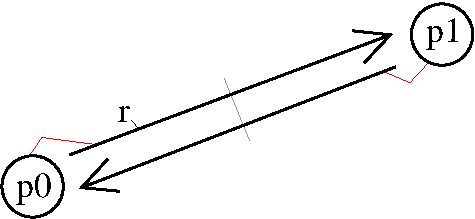
\includegraphics[width=\LargFig]{Linear_cell_complex_ref/fig/pdf/make_segment}
  \end{center}
\end{ccTexOnly}
\begin{ccHtmlOnly}
  <CENTER>
  <A HREF="fig/png/make_segment.png">
  <img src="../Linear_cell_complex_ref/fig/png/make_segment.png" alt=""></A>
  </CENTER>
\end{ccHtmlOnly}
\centerline{Example of \ccc{r=lcc.make_segment(p0,p1)}.}

\ccMethod{Dart_handle make_triangle(const Point& p0, const Point& p1, const Point& p2);}  
{Creates an isolated triangle in \ccc{lcc} having \ccc{p0}, \ccc{p1}, \ccc{p2} as points.
   Returns a handle on the dart associated with \ccc{p0}.
 \ccPrecond{\ccc{dimension}\mygeq{}1.}
}
%
\def\LargFig{.3\textwidth}
  \begin{ccTexOnly}
    \begin{center}
      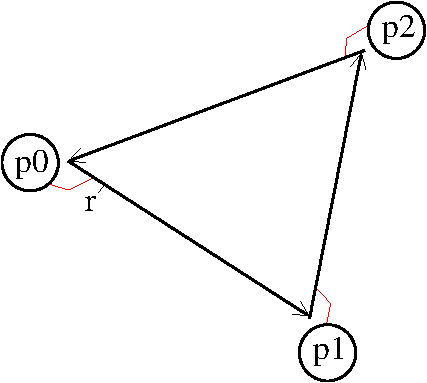
\includegraphics[width=\LargFig]{Linear_cell_complex_ref/fig/pdf/make_triangle}
    \end{center}
  \end{ccTexOnly}
  \begin{ccHtmlOnly}
    <CENTER>
    <A HREF="fig/png/make_triangle.png">
        <img src="../Linear_cell_complex_ref/fig/png/make_triangle.png" alt=""></A>
    </CENTER>
    \end{ccHtmlOnly}
    \centerline{Example of \ccc{r=lcc.make_triangle(p0,p1,p2)}.}

\ccMethod{Dart_handle make_quadrangle(const Point& p0,const Point& p1,const Point& p2,const Point& p3);}  
{Creates an isolated quadrangle in \ccc{lcc}  having \ccc{p0}, \ccc{p1}, 
  \ccc{p2}, \ccc{p3} as points.
   Returns a handle on the dart associated with \ccc{p0}.
 \ccPrecond{\ccc{dimension}\mygeq{}1.}
}
%
\def\LargFig{.3\textwidth}
  \begin{ccTexOnly}
    \begin{center}
      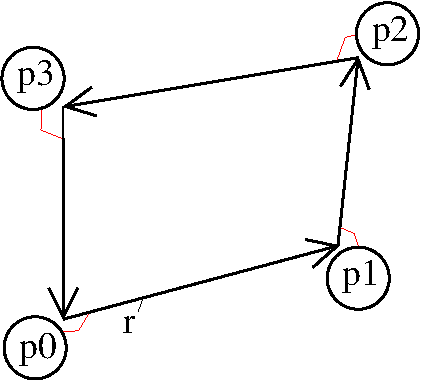
\includegraphics[width=\LargFig]{Linear_cell_complex_ref/fig/pdf/make_quadrilateral}
    \end{center}
  \end{ccTexOnly}
  \begin{ccHtmlOnly}
    <CENTER>
    <A HREF="fig/png/make_quadrilateral.png">
        <img src="../Linear_cell_complex_ref/fig/png/make_quadrilateral.png" alt=""></A>
    </CENTER>
    \end{ccHtmlOnly}
    \centerline{Example of \ccc{r=lcc.make_quadrangle(p0,p1,p2,p3)}.}

\ccMethod{Dart_handle make_tetrahedron(const Point& p0,const Point& p1,const Point& p2,const Point& p3);}
{Creates an isolated tetrahedron in \ccc{lcc} having \ccc{p0},
  \ccc{p1},\ccc{p2},\ccc{p3} as points.  Returns a handle on the dart
  associated with \ccc{p0} and belonging to the 2-cell having
  \ccc{p0}, \ccc{p1}, \ccc{p2} as points.
  \ccPrecond{\ccc{dimension}\mygeq{}2.}  }
%
\def\LargFig{.3\textwidth}
  \begin{ccTexOnly}
    \begin{center}
      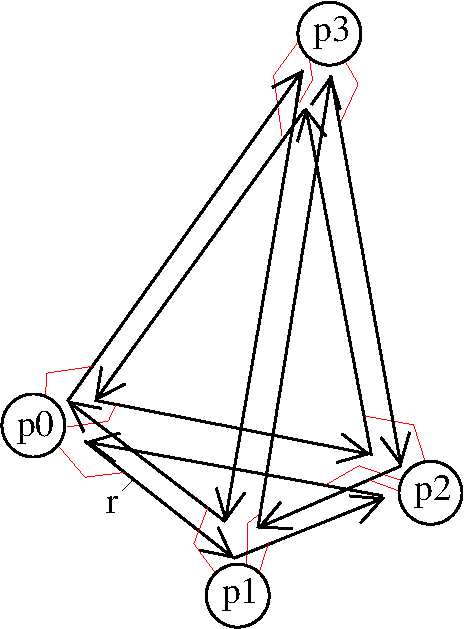
\includegraphics[width=\LargFig]{Linear_cell_complex_ref/fig/pdf/make_tetrahedron}
    \end{center}
  \end{ccTexOnly}
  \begin{ccHtmlOnly}
    <CENTER>
    <A HREF="fig/png/make_tetrahedron.png">
        <img src="../Linear_cell_complex_ref/fig/png/make_tetrahedron.png" alt=""></A>
    </CENTER>
    \end{ccHtmlOnly}
    \centerline{Example of \ccc{r=lcc.make_tetrahedron(p0,p1,p2,p3)}.}

\ccFunction{Dart_handle make_hexahedron(const Point& p0,const Point& p1,const Point& p2,const Point& p3,const Point& p4,const Point& p5,const Point& p6,const Point& p7);}
{Creates an isolated hexahedron in \ccc{lcc} having \ccc{p0}, \ccc{p1},
\ccc{p2}, \ccc{p3}, \ccc{p4}, \ccc{p5}, \ccc{p6}, \ccc{p7} as points.
  Returns a handle on the dart associated with \ccc{p0} and
  belonging to the 2-cell having \ccc{p0}, \ccc{p5}, \ccc{p6}, \ccc{p1}
  as points.
  \ccPrecond{\ccc{dimension}\mygeq{}2.}
}
\def\LargFig{.4\textwidth}
  \begin{ccTexOnly}
    \begin{center}
      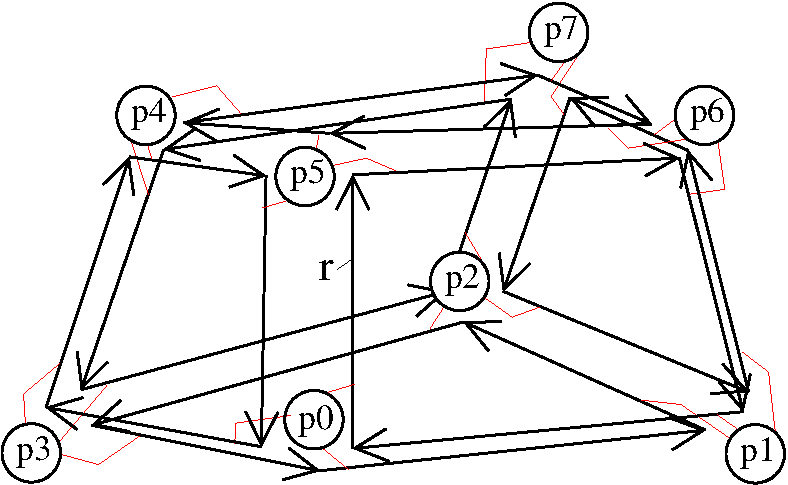
\includegraphics[width=\LargFig]{Linear_cell_complex_ref/fig/pdf/make_hexahedron}
    \end{center}
  \end{ccTexOnly}
  \begin{ccHtmlOnly}
    <CENTER>
    <A HREF="fig/png/make_hexahedron.png">
        <img src="../Linear_cell_complex_ref/fig/png/make_hexahedron.png" alt=""></A>
    </CENTER>
    \end{ccHtmlOnly}
    \centerline{Example of \ccc{r=lcc.make_hexahedron(p0,p1,p2,p3,p4,p5,p6,p7)}.}

% +-----------------------------------+
\ccSeeAlso
\ccRefConceptPage{CombinatorialMap}\\
\ccRefIdfierPage{CGAL::Combinatorial_map<d,Items,Alloc>}\\
\ccRefConceptPage{Dart}\\
\ccRefConceptPage{LinearCellComplexItems}\\
\ccRefIdfierPage{CGAL::Linear_cell_complex_min_items<d>}\\
\ccRefConceptPage{LinearCellComplexTraits}\\
\ccRefIdfierPage{CGAL::Linear_cell_complex_traits<d,K>}

\end{ccRefClass}
% +------------------------------------------------------------------------+
%%RefPage: end of main body, begin of footer
\ccRefPageEnd
% EOF
% +------------------------------------------------------------------------+
